\chapter{ROS}

The software system controlling the rover and processing the incoming sensor data is built on top of the Robot Operating System (ROS). ROS is a meta operating system for open-source robotics. It provides an asynchronous messaging framework for multiple processes to communicate across multiple machines, package management for shared robotics libraries, and makes it easy to handle multiple moving coordinate systems.

\section{ROS Basics}

\subsection{Messaging}

Processes in ROS are known as nodes. Nodes communicate by publishing and subscribing to certain communication channels called topics. The data passed over these topics are various classes of rigidly defined data structures called messages. Messages often contain meta-data such as a timestamp and sequence number, in addition to the data of interest.

When a node publishes a message to a particular topic, all nodes subscribed to that topic receive a copy. Any number of processes may publish or subscribe to a topic, making this a many-to-many communication protocol. Under the hood, messaging between nodes is handled by the ROS Master node, which acts like a DNS server and must be running for the ROS system to function. 

We will use a simple example to illustrate. Assume a fresh ROS system, with only two nodes: A and B. If node A wishes to subscribe to messages coming from topic "/foo", it will register its intent with the Master. Then, if node B starts publishing messages to topic "/foo", it will also register this with the Master. When node B does so, the Master node will notify all registered subscribers on the "/foo" topic. Node A will receive the TCP/IP socket address of Node B, and communicate directly to negotiate opening a socket. Then each time node B publishes a message to "/foo", it will iterate through its list of connected sockets nodes, and push message data through each one. Every time the list of registered subscribers or publishers for topic "/foo" is updated, the Master node notifies all nodes registered to that topic.

\subsection{Packages}
Packages are collections of related ROS resources which all work together to perform some specific task. They often include source code for nodes, executable utilities, message definitions, and launch files. There are also meta-packages which collect various related packages.

Launch files are XML files which define several nodes to be run at once. Robotics systems grow large quickly, and require many nodes. This project ended up using 12 nodes throughout its launch files. Manually starting all of those nodes would be tedious, and launch files automate that process. They also allow convenient parameter specification for each node. Parameters are stored in separate files, and are loaded dynamically when a launch file is run.

\subsection{Frames and Transforms}

Robotics systems include many moving parts. In order to keep track of those parts and their relation to one another, many different coordinate axes are needed. In ROS, these coordinate axes are called frames, and just like topics they are each given a unique name. The rover works with five frames in total, and follows the standards specified in REP-103 and REP-103 \cite{REP-103} \cite{REP-105}.
% http://www.ros.org/reps/rep-0103.html
% http://www.ros.org/reps/rep-0105.html

%There are two main pieces to consider when asking where the rover is: its position, and its orientation.

The basic starting frame is the "base\_link" frame, which has its origin at the center of the rover. This frame is rigidly attached, and follows the translation and rotation of the rover. The X axis of the base\_link frame always points forward, the Y axis points to the robot's left, and the Z axis points straight up above the robot.

Next we define a frame for the smartphone, simply called phone. The phone frame has its origin at the center of the phone, roughly two inches to the right of the base\_link frame. This frame is once again attached, and moves with the translation of the smartphone. However, while the origin shifts, the orientation of the axes stays constant with respect to the earth. The X axis always points east, its Y axis points north, and its Z axis points up towards the sky, or tangential to the earth's surface. This axis orientation is referred to as the ENU convention (East-North-Up).

Another frame needed is a frame fixed to the local environment. The origin and orientation of this frame should be the same as the base\_link frame initially: origin at the center, X axis forward, Y to the left, and Z up. However, this frame will not be rigidly attached to the rover body, and will not move or rotate as the rover moves. Thus it will be able to keep track of the rover's total movement from its starting position.

We will define two such locally fixed frames: odom and map. We will use the map frame to keep track of the position estimate of the rover using all available sensors, including GPS. The GPS measurements filtered through the EKF will cause this estimate to jump around erratically, making it discontinuous. We will use the odom frame to keep track of the position estimate of the rover, using all sensors except for the GPS. This position estimate will be smooth and continuous, but the position error will grow unbounded over time.

\begin{figure}[h]
	\caption{\cite{robot_localization_wiki}}
	\label{fig:roverFrames}
	\centering
	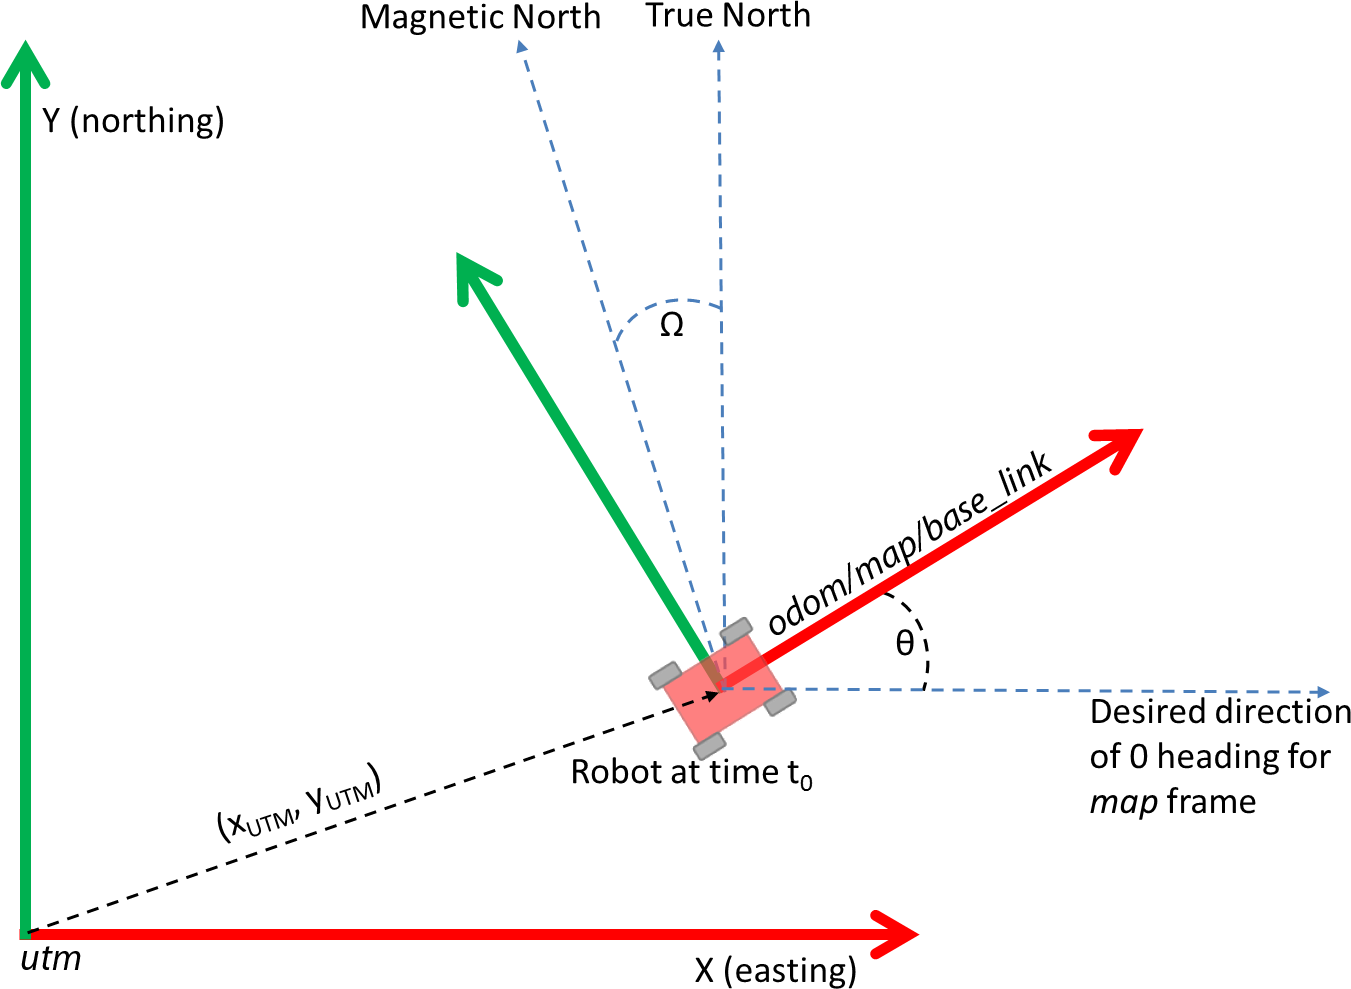
\includegraphics[width=\textwidth]{roverFrames}
\end{figure}

The UTM (Universal Transverse Mercator) frame defines a frame equal to the axes used by the UTM zone that the rover is currently in. The origin is at the (0,0) point of the UTM zone, and the axes are oriented according to the ENU convention. See Figure \ref{fig:roverFrames} for a graphical representation of the UTM frame compared to the other frames. The figure shows the rover at time \(t = 0\), right at the start of localization. Notice that the base\_link, odom, and map frames are all aligned. The phone frame, not pictured, would have the same origin as those three, but its axes would be oriented parallel to the UTM frame's axes. As the rover moves, the base\_link and phone frames would move with it. The base\_link axes would rotate as the rover rotates, and the phone axes would remain oriented as ENU. The odom and map frames would stay fixed at where they began. 

\begin{wrapfigure}{R}{0.5\textwidth}
	\caption{Transforms}
	\centering
	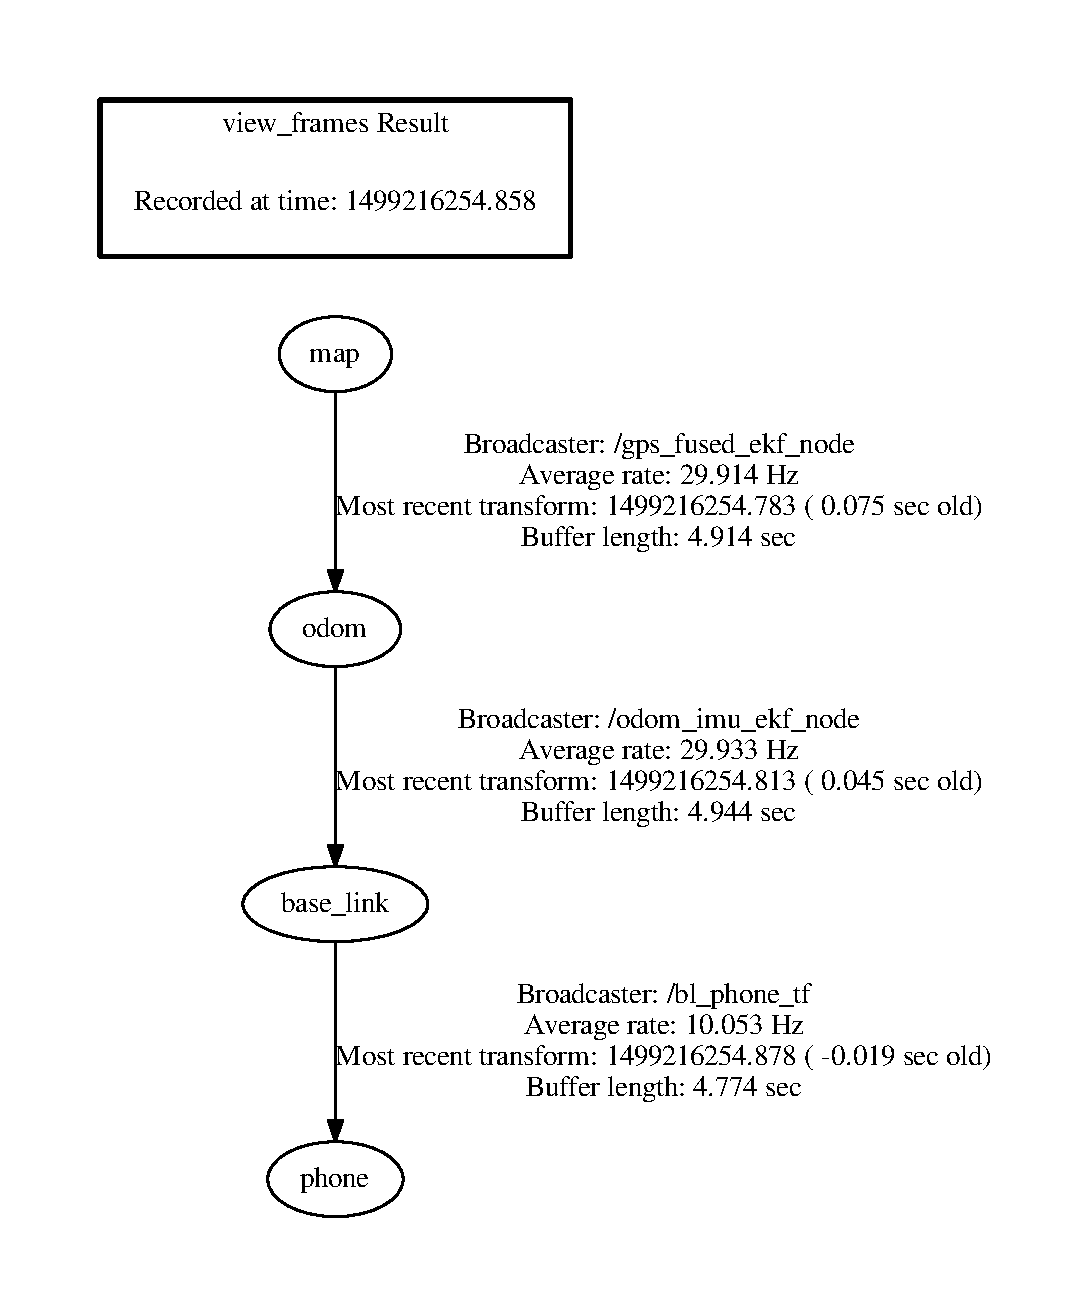
\includegraphics[width=0.5\textwidth]{frames}
	\label{fig:frames}
\end{wrapfigure}

As the rover localizes, it calculates its position with respect to the odom, map, and utm frames. Odometry data coming from the wheel encoders is reported with respect to the base\_link frame, while IMU and GPS sensor data from the phone is reported w.r.t. the phone frame. For the rover to fuse this data together, it needs to transform it into the equivalent information in one of the fixed frames: odom or map. 

ROS supplies convenient tools for handling these transforms. The \(tf\) package allows nodes to broadcast transform definitions through the ROS network. See Figure \ref{fig:frames} for a map of all transforms broadcast in this system, where arrows indicate a transform converting a parent frame to a child frame.

\section{rosserial} \label{sectionRosSerial}
Communication between the Arduino and laptop is handled by the ROS meta-package rosserial. Different client packages support different client machines, such as embedded linux devices, or different microcontroller boards. These client packages create local support libraries or header files on those machines, which use a serialization protocol to send and receive ROS messages over a serial port. On the other side of the serial connection, host packages run a bridging node which communicates with the ROS network on behalf of the client machine. Subscribed topics have their messages serialized and sent to the client machine, and outgoing messages from the client are de-serialized and published. 

\subsection{rosserial\_arduino}
rosserial\_arduino is one client package of rosserial, which creates an Arduino library to provide bare-bones ROS support to sketches. The sketch running on this project's Uno board uses this library to publish sensor data in ROS messages, and subscribe to motor command topics.

Every time the sketch wishes to update the laptop with its newest sensor readings, it publishes three messages. First the servo angle in degrees is published to the "/ping/angleDeg" topic, as a standard Int8 message. This message just contains a single data field: an 8-bit signed integer. Next the echo time in microseconds is published to the "/ping/timeUS" topic, as a standard UInt16 message which contains a single 16 bit data field representing an unsigned integer. Lastly the two encoder tick counts are both placed into a single custom message called EncCount, and published to the "/odom/encTicks" topic. This custom message type has two 32 bit fields, one for each encoder.

When the sketch is waiting between updates, it continually listens to the serial port for motor commands. These commands are Int8 messages on the "/cmd/left" or "/cmd/right" topics, which the sketch subscribes to. When these messages are found in the serial input buffer, a short callback function is executed, which writes the R/C pulse command to the proper motor channel.

Arduino boards use different types of memory. Flash memory is used to store compiled code, and static random access memory (SRAM) is used to store dynamic variables at runtime. The Uno has 32kB of flash memory, but only 2kB of SRAM. The rosserial\_arduino library is large, and takes up quite a lot of SRAM space. Its input and output serial buffers alone use 1024 bytes in total. This makes running out of space for local variables quite easy, which can lead to instability and crashes when running the sketch. To save space, a modified version of rosserial\_arduino has been used, which supports storing constant strings in flash memory rather than SRAM. Since topic names and error messages use long descriptive strings, this saves several hundred kB of space in SRAM and ensures the sketch's stability.
%https://github.com/strothmw/rosserial

The library abstracts away most of the serial communication protocol, but does allow the baud rate to be specified. In this use case, baud rate is equivalent to bits per second. The more bits per second sent over serial, the more frequently the microcontroller needs to sample the incoming and outgoing line. So the baud rate cannot be set arbitrarily high, as the Uno has a limited clock speed. If it is set too low, however, then the stream of sensor data being published would overwhelm the connection. Significantly less data will be streaming in than transmitted out, so the amount of outgoing data is the deciding factor. Thus to calculate an appropriate baud rate, the amount of sensor data transmitted per second must be known.

Communication between board and laptop involves a serial protocol with 8 bytes of overhead for every message. Each sensor update publishes three messages: an eight-byte EncCount message, a one-byte Int8 message, and a two-byte UInt16 message. This means that each update pushes 11 bytes of data in three messages, with 24 bytes of overhead. Thus a total of 35 bytes are sent over serial.

Since the PING))) sensor requires a minimum delay of 30 ms between pings, the sketch cannot publish its sensor values at a rate higher than 33 Hz. Therefore the sketch will not push more than:
\[33\ Hz * 35\ Bytes = 1155\ Bytes\ per\ second\ (Bps)\]

The Uno uses one start bit and one stop bit to surround each byte of information sent over serial. Thus it takes 10 bits to send one byte of information. Therefore the minimum baud rate required is:
\[1155\ Bps * 10\ bits\ per\ byte = 11550\ bits\ per\ second\]

We choose a standard baud rate of 28,800 to more than double that for some breathing room, and to account for the fact that the rosserial Arduino library occasionally transmits time-keeping and synchronization messages of its own.

\subsection{rosserial\_python}
rosserial\_python is one host package of rosserial, which acts as a bridge between the Arduino and ROS network. It runs a node on the laptop which communicates with the Arduino using the rosserial protocol. It automatically handles setup, communication with the ROS Master, and subscription and publishing on behalf of the Arduino. When launched, the serial node must be configured to use the same baud rate as the Arduino: 28,800. It must also be configured to connect to whichever serial port name the Arduino uses. For simplicity, a symbolic link was created using Ubuntu's udev rules, to ensure that the port name will always be accessible as "/dev/arduino". %https://www.clearpathrobotics.com/2015/01/arduino-ros/

\section{differential\_drive}
The differential\_drive package was created by Jon Stephan to create a simple interface for controlling a differential wheeled robot \cite{differentialDrivePackage}. Such a robot uses a two-wheeled system where both wheels are on a common axis, but each wheel is driven independently. Turning is achieved by lowering the velocity of one wheel compared to the other.

Because the rover has four wheels, turning necessarily involves slippage of one or more wheels. This is known as a skid-steering system, due to the skidding of the wheels. When wheels slip, they move without rotating. The motor encoders cannot see this movement, and so this causes error in the wheel odometry estimate, especially in the rover's heading. Despite this flaw, the differential\_drive package was used to model the rover as a differentially steered robot for the purposes of dead reckoning, due to the lack of a better option within ROS.

\subsection{diff\_odom} \label{sectionOdomPublishing}

Odometry messages are a type of ROS message used for navigation. They represent an estimate of the position and velocity of the rover at a certain time. The diff\_odom node subscribes to encoder tick data, and uses that data to calculate and publish an Odometry message to the "odometry/wheel" topic. The Odometry messages contain estimates of the rover's position, orientation, and linear and angular velocity with a timestamp. This node is a modified version of the diff\_tf node from the differential\_drive package, which was changed to use the custom EncCount message type, set appropriate covariance values, and not publish an odom->base\_link transform. That transform is published by the EKF node after fusing all sensor data, as will be described in section \ref{sectionRobotLocalization}.

\begin{figure}[h]
	\caption{\cite{differentialSteeringPaper}}
	\centering
	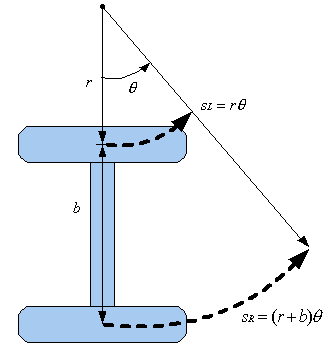
\includegraphics{diff_drive}
	\label{figDiffDrive}
\end{figure}

To understand how the diff\_odom node calculates its odometry estimate, let us take a look at the standard theory for differential wheeled robots. Figure \ref{figDiffDrive} shows a simple two-wheeled robot making a left turn of \(\theta\) radians around some point. We assume the robot is one rigid body, and that each wheel maintains a constant velocity along the turn. This assumption of zero acceleration is obviously violated in the real world, but robots with a small mass and relatively powerful motors are able to approximate it well. \cite{differentialSteeringPaper}

\(r\) is the turning radius for the left wheel, and \((r+b)\) is the turning radius for the right wheel, where \(b\) is the distance between wheels. Using the formula for arc length, we know the distance traveled by the right and left wheels. Define these to be \(s_L\) and \(s_R\). Then let point M be the midpoint of the axle between both wheels. This point will travel an arc length of \((r+(b/2)) \theta \). We can manipulate \(s_L\) and \(s_R\) to produce the following two equations.
\begin{equation} \label{eqDiffSM}
s_M = ((r+(b/2)) \theta = \frac{(2r + b) \theta}{2} = \frac{(r + b)\theta + r \theta}{2} = \frac{(s_L + s_R)}{2}
\end{equation}
\begin{equation} \label{eqDiffTheta}
\theta = \frac{b\theta}{b} = \frac{(b + r - r) \theta}{b} = \frac{((r+b) \theta - r \theta)}{b} = \frac{(s_R - s_L)}{b}
\end{equation}

Equation \ref{eqDiffSM} gives the distance the center of the robot travels over the turn, in terms of the distance the two wheels traveled. Dividing this distance by the elapsed time it took to make the turn, gives an estimate of the instantaneous velocity of the robot at the end of the turn. Similarly, equation \ref{eqDiffTheta} calculates the angle of the turn using the distance the two wheels traveled. Dividing \(\theta\) by the elapsed time gives the angular velocity of the robot.

Both calculations make use of the distance traveled by the two wheels. The two motor encoders attached to the rover's front wheels report a known number of ticks per revolution, and the wheel circumference can be calculated from the wheel diameter. Thus the distance each wheel travels can be computed using the difference of encoder ticks between sensor updates. The diff\_odom node uses these distances and equations \ref{eqDiffSM} and \ref{eqDiffTheta} to calculate the rover's angular and linear velocity. Only the angular velocity along the rover's Z axis is reported; the wheel odometry says nothing about the angular velocity along the other axes. Because a differentially steered robot can only move in the direction of its fixed wheels, the linear velocity is reported along the base\_link X axis, which faces forward from the rover's midpoint.

The Odometry message published includes a \(6 \times 6\) covariance matrix for the linear and angular velocities along all three axes. These covariances will give the EKF an idea of how much confidence to place in these velocity estimates. Since only two velocities are calculated, constant squared variances are hard-coded in for those two variables along the matrix diagonal. Every other element in the covariance matrix is set to zero. The Odometry message also includes a pose element, which is a position in the odom frame. However, due to the inaccuracy of the differential drive approximation made, this estimate quickly becomes rather useless. So the EKF is configured to ignore the pose from this Odometry message completely. The odometry messages are published at a rate equal to the Arduino's sensor update rate: 10 Hz. If it were published at a slower rate, then some resolution would be lost as encoder tick messages would be skipped over.

Though the number of encoder ticks per meter may be calculated from the encoders' specification and the diameter of the wheels, it is a good idea to manually calibrate the number of encoder ticks per meter, and specify this as a configurable parameter to the diff\_odom node. This helps account for sources of error in the physical system. The ticks per meter can easily be calibrated by moving the Arduino one meter, and comparing the starting and ending tick count.

\subsection{twist\_to\_motors}
Many ROS navigation packages produce Twist messages to command robotic platforms. The Twist message includes a linear and angular velocity, which the rover is expected to match, as a subfunction of some path following algorithm. The differential\_drive package uses the twist\_to\_motors node to translate Twist messages into individual motor velocities for each motor channel. 

Taking into account the differentially steered conditions, this node only considers the linear velocity along the rover's x axis, and the angular velocity around the rover's z-axis. Let us refer to these as \(x'\) and \(\theta '\), respectively. Let \(b\) once again be the distance between the rover's wheels. Let \(L'\) and \(R'\) be the velocity of the left and right wheels. From equation \ref{eqDiffSM}, we know that
\begin{equation*}
x' = (L' + R') / 2
\end{equation*}
and from equation \ref{eqDiffTheta} we know that
\begin{equation*}
\theta ' = (R' - L') / b
\end{equation*}

This is a system of two equations with two unknowns, \(L'\) and \(R'\). Solving this system gives us: 
\begin{align*}
L' = x' - (b * \theta ') / 2 \\
R' = x' + (b * \theta ') / 2
\end{align*}

This node uses these equations to calculate the appropriate wheel velocities from the incoming Twist message, and publishes those velocities to the "lwheel\_vtarget" and "rwheel\_vtarget" topics. 

\subsection{pid\_velocity}
The pid\_velocity node creates a  proportional-integral-derivative (PID) controller which uses encoder feedback to translate motor velocities into actual motor R/C pulse commands. While the appropriate R/C servo command to reach a desired velocity could be estimated from the Sabertooth motor driver's datasheet, this would be the theoretical value and would not take into account real-world sources of error such as uneven terrain, high traction, wind drag, etc. Therefore a control loop which utilizes real-time feedback is preferred.

Two of these nodes are run, one for each motor channel. One node subscribes to the topic "lwheel\_vtarget", and publishes commands to "/cmd/left", while the other node subscribes to "rwheel\_vtarget", and publishes to "/cmd/right". The Arduino node, through its bridge, is subscribed to these two topics and handles their messages appropriately.

PID controllers work by adjusting their output according to an error term, which is the difference between the current feedback and the desired value. In this case the error is the difference between the wheel velocity published by the diff\_odom node, and the target wheel velocity. This error, the integral of all past errors, and the instantaneous derivative of the current error are all combined into a weighted sum. This sum then acts as the new output of the system.

The weights in the sum are three constant parameters: \(K_p\), \(K_i\), and \(K_d\). These parameters must be manually tuned to the target system for optimal use of the controller. The tuning procedure involves zeroing out \(K_i\) and \(K_d\), and slowly increasing \(K_p\) until oscillation is observed in the control loop. Once a limit is found, set \(K_p\) to half of it. Then tune \(K_i\) and lastly \(K_d\), in the same fashion. 

\subsection{virtual\_joystick} \label{sectionJoystick}
For testing of the rover's localization capabilities, it was necessary to manually drive it. This was accomplished using the virtual\_joystick node from the  differential\_drive package. To use the node, one must install PySide, the python binding for the GUI framework Qt. The node brings up a simple GUI, and allows the user to drag their mouse along a two-dimensional axis. This axis represents a desired linear and angular velocity, and the node publishes a corresponding Twist message. This node will not be needed once autonomous navigation is fully functional.

\section{Ros Sensors App}
In order to access the smartphone's IMU and GPS data, an Android app was written to act as a ROS node. All sensor messages published are from the phone's frame, which is centered 2 inches to the right of the base\_link frame, and always has the ENU orientation. The app makes use of phone tethering supported by the Android OS, which allows one to access the internet over a smartphone's data plan. However, this feature is used only as a convenient way for the phone and laptop to communicate locally over USB.

\subsection{GPS}
\begin{wrapfigure}{L}{0.5\textwidth} 
	\caption{Trilateration \cite{GPS_trilateration}}
	\centering
	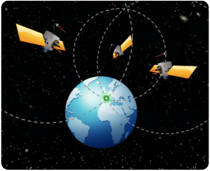
\includegraphics[width=0.25\textwidth]{trilateration}
\end{wrapfigure}

The Global Positioning System (GPS) was developed by the U.S. Department of Defense, and has been operational since 1995. It currently involves 31 satellites orbiting the earth in such a way that four or more satellites are always visible from most land masses. Each satellite broadcasts a signal via radio wave, which contains the exact time the signal was sent, as well as orbital information about the exact position of the satellite at that time. When a GPS receiver reads one of these signals, it looks at the current time and calculates the length of time the signal took to reach the receiver. It can then multiply this length by the speed of light to calculate the distance between the receiver and satellite. This distance can be thought of as the radius of a sphere centered at the satellite. The receiver must be somewhere on that sphere. Because four spheres can only intersect at one point, if the receiver knows its distance from four satellites, then it can calculate the intersection point - its location with respect to the earth. This process is known as trilateration. \cite{GPS_trilateration}

The GPS coordinates reported by the phone node are acquired using assisted GPS (AGPS). In AGPS, cell phone towers use a phone's signal strength to help determine its position. This provides quicker and more precise location tracking. At greater cost, one could purchase GPS hardware to access gps fix messages broadcast by the coastguard for even greater precision.

The phone node publishes gps messages as they come in: roughly every five seconds. The covariance matrix is filled in along the diagonal, using the variances reported by the Android OS.

\subsection{IMU}

Inertial Measurement Units (IMUs) are small chips that measure linear and angular movement. A digital accelerometer measures linear acceleration in all three dimensions, while a digital gyroscope measures angular velocity around each axis. Lastly, a digital magnetometer measures magnetic strength along each axis. IMU chips often report their data in the NED (North-East-Down) orientation, however the Android API reports values using the ENU convention, as expected. A covariance matrix was once again filled out on only the diagonals, with squared variances hard-coded at reasonable estimates. All of this information is encapsulated in a ROS IMU message, which is published at approximately 5 Hz. 

\section{robot\_localization} \label{sectionRobotLocalization}
%http://docs.ros.org/kinetic/api/robot_localization/html/

\begin{wrapfigure}{R}{0.5\textwidth} 
	\caption{Roll, Pitch, and Yaw \cite{fig_rpy}}
	\label{fig:rpy}
	\centering
	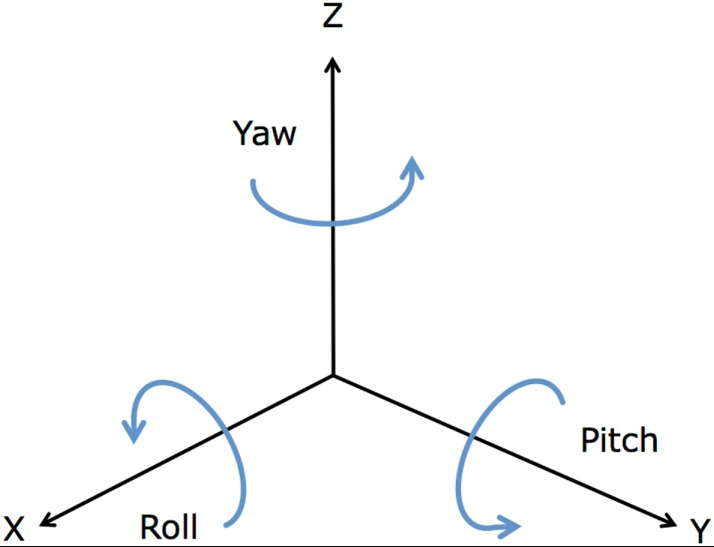
\includegraphics[width=0.25\textwidth]{rpy}
\end{wrapfigure}

This package created by Tom Moore implements the extended Kalman Filter, which was derived in section \ref{sectionEKF}. The filter keeps track of a 15-dimensional vector describing the rover's state: \((x,y,z,\Phi,\theta,\Psi,x',y',z',\Phi ',\theta ',\Psi ', x'', y'', z'')\) \cite{robot_localization_paper}. In this state vector  \(\Phi\), \(\theta\), and \(\Psi\) represent roll, pitch, and yaw respectively. These Euler angles describe rotation about the X, Y, and Z axes. See Figure \ref{fig:rpy} for an illustration. 

This project takes advantage of the fact that the rover is a ground vehicle and makes the assumption that all terrain is perfectly flat, and that the rover is moving in a two-dimensional environment. Thus z, roll, pitch, and their derivatives in the state vector are fixed at 0. This configuration should be changed for more elaborate testing, however this assumption eliminates an entire axis of noise from GPS altitude and IMU measurements. 

\definecolor{Gray}{gray}{0.85}
\newcolumntype{a}{>{\columncolor{Gray}}c}
\newcolumntype{b}{>{\columncolor{white}}c}
\begin{table}
	\caption {Sensor Configurations \cite{robot_localization_paper}}
	\label{tab:configs}
	\begin{center}
		\begin{tabular}{|l|a|b|a|b|a|b|a|b|a|b|a|b|a|b|a|} \hline
			\theadfont\diagbox[width=11em]{Sensor}{State\\Variable}&
			\textbf{\(x\)} & \textbf{\(y\)} & \textbf{\(z\)} & \textbf{\(\Phi\)} & \textbf{\(\theta\)} & \textbf{\(\Psi\)} & \textbf{\(x'\)} & \textbf{\(y'\)} & \textbf{\(z'\)} & \textbf{\(\Phi '\)} & \textbf{\(\theta '\)} & \textbf{\(\Psi '\)} & \textbf{\(x''\)} & \textbf{\(y''\)} & \textbf{\(z''\)} \\ \hline
			%\thead{Second\\column}&\thead{Third\\column}\\    \hline
			Wheel Encoders & 0 & 0 & 0 & 0 & 0 & 0 & 1 & 0 & 0 & 0 & 0 & 1 & 0 & 0 & 0 \\    \hline
			IMU & 0 & 0 & 0 & 0 & 0 & 0 & 0 & 0 & 0 & 1 & 1 & 1 & 1 & 1 & 0 \\ \hline
			GPS & 1 & 1 & 0 & 0 & 0 & 0 & 0 & 0 & 0 & 0 & 0 & 0 & 0 & 0 & 0 \\ \hline
		\end{tabular}
	\end{center}
\end{table}

Table \ref{tab:configs} shows which state variables each sensor affects, where a 1 indicates that the sensor gives a reading for the corresponding state variable, and a 0 indicates that it does not.

The rover's system runs three nodes from this package. The first node runs an EKF which fuses wheel odometry from the diff\_odom node (section \ref{sectionOdomPublishing}) with IMU data from the phone node. It produces a state estimate in the odom frame.

The second node provides a helper service that transforms gps coordinates into a locally fixed frame, and vice versa. Its main use is to transform gps messages coming from the phone node into coordinates in the map frame.

The third and final node runs another EKF which fuses the odometry output from the first and second nodes together, producing a final  state estimate in the map frame. This estimate is discontinuous, as the output from the second node is positional coordinates, which this node uses to instantaneously adjust the rover's \(x\) and \(y\) state variables.